\documentclass[12pt,a4paper,titlepage]{scrreprt}

% Language is defined in package module

\usepackage {fontspec}
\usepackage[hidelinks]{hyperref}
\usepackage{pdfpages} % For inclusion of PDFs

\usepackage{tabulary}
\usepackage{emoji}

%pro formátování čísel
\usepackage{numprint}
\npthousandsep{\,}\npthousandthpartsep{}\npdecimalsign{.}

%Uprava (odstraneni modifikaci generovaneneho texttu tridou scratcl)
\setkomafont{disposition}{\mdseries\rmfamily}

\title{\vspace{6cm}Návrh zařízení pro testování nabíjecích kabelů}
\subtitle{Bakalářská práce}
\author{Filip Šimek}
\date{\today}

\hypersetup{
	pdfauthor={Filip Šimek},%
	pdftitle={Návrh zařízení pro testování nabíjecích kabelů},%
	pdfsubject={Bakalářská práce},%
	%pdfkeywords={one, two},%
	%pdfproducer={LaTeX},%
	pdfcreator={LuaLaTeX}
}

%font
\setmainfont{Times_New_Roman}

%Rozestup řádku (1.5)
%\linespread{1.35}
%\linespread{1.5}
\linespread{1.25}

%Nastaveni okraje (normostrana)
\usepackage[a4paper, left=3.50cm, right=1.50cm, top=2.50cm, bottom=2.50cm]{geometry}

\RedeclareSectionCommand[
  beforeskip=.1cm,
  afterskip= .1cm %1.0ex plus .2ex
]{chapter}

%\setkomafont{chapter}{\fontsize{18}{18*1.2}\selectfont}
\setkomafont{chapter}{\fontsize{16}{19.2}\selectfont}   
\setkomafont{section}{\fontsize{14}{16.8}\selectfont}
\setkomafont{subsection}{\fontsize{13}{15.6}\selectfont}
\setkomafont{subsubsection}{\fontsize{13}{15.6}\selectfont}

\makeatletter
\newcommand\thefontsize{(Font size = \f@size pt)}
\makeatother

% WIP modules
%\usepackage{glossaries}
%%!TeX root =  ../thesis.tex

\makeglossaries

\newglossaryentry{keyword1}{
    name={Keyword 1},
    description={Description of Keyword 1}
}

\newglossaryentry{keyword2}{
    name={Keyword 2},
    description={Description of Keyword 2}
}

\newglossaryentry{ard}{
    name={Arduino},
    description={IoT device}
}
%\makeglossaries

% My modules
% Přidá automatické zalomení spojek

%\usepackage[czech]{babel}
\usepackage{polyglossia}
\setdefaultlanguage{czech}

% Define custom hyphenation rules
%\babelhyphenation[czech]{a}
%\babelhyphenation[czech]{u}
%\babelhyphenation[czech]{i}
%\babelhyphenation[czech]{v}
%\babelhyphenation[czech]{s}
%\babelhyphenation[czech]{o}
%\babelhyphenation[czech]{proto}
%\babelhyphenation[czech]{protože}
%\babelhyphenation[czech]{je}
% Přidá article příkaz pro drobnější dělení

\makeatletter
\renewcommand\paragraph{\@startsection{paragraph}{4}{\z@}%
            {-2.5ex\@plus -1ex \@minus -.25ex}%
            {1.25ex \@plus .25ex}%
            {\normalfont\normalsize}}
\makeatother
\setcounter{secnumdepth}{4} % how many sectioning levels to assign numbers to
\setcounter{tocdepth}{4}    % how many sectioning levels to show in ToC
% Přidá custom zvýraznění v listings

\usepackage{listings}
\usepackage{xcolor}

\definecolor{codegreen}{rgb}{0,0.6,0}
\definecolor{codegray}{rgb}{0.5,0.5,0.5}
\definecolor{codepurple}{rgb}{0.58,0,0.82}
\definecolor{backcolour}{rgb}{0.95,0.95,0.92}

\lstdefinestyle{mystyle}
{
morekeywords={override}, % Add 'override' as a keyword
backgroundcolor=\color{backcolour},   
commentstyle=\color{codegreen},
keywordstyle=\color{magenta},
numberstyle=\tiny\color{codegray},
stringstyle=\color{codepurple},
basicstyle=\footnotesize,
breakatwhitespace=false,         
breaklines=true,                 
captionpos=b,                    
keepspaces=true,                 
numbers=left,                    
numbersep=5pt,                  
showspaces=false,                
showstringspaces=false,
showtabs=false,                  
tabsize=2,
escapeinside=``
}

\lstset
{
morekeywords={override}, % Add 'override' as a keyword
style=mystyle
}
% Přidá tabulky++

\usepackage{multirow}
\usepackage{makecell}
\usepackage{array}
%Justify text mode
\tolerance=1
\emergencystretch=\maxdimen
\hyphenpenalty=10000
\hbadness=10000

% My commands
\newcommand{\ardMeg}{Arduino Mega 2560}

\begin{document}

	%\includepdf{specialPages/frontPage/frontPage.pdf} %Desky
	\includepdf{specialPages/titlePage/titlePage.pdf} %\maketitle 
	\includepdf[pages={1-2}]{specialPages/zadaniBP.pdf}
	
	%!TeX root =  ../thesis.tex

Prohlašuji: \\
Práci s názvem “Návrh zařízení pro testování nabíjecích kabelů” jsem vypracoval samostatně. Veškeré literární prameny a informace, které jsem v práci využil, jsou uvedeny v seznamu použité literatury.
Byl jsem seznámen s tím, že se na moji práci vztahují práva a povinnosti vyplývající ze zákona č. 121/2000 Sb., o právu autorském, o právech souvisejících s právem autorským a o změně některých zákonů (autorský zákon), ve znění pozdějších předpisů, zejména se skutečností, že Univerzita Pardubice má právo na uzavření licenční smlouvy o užití této práce jako školního díla podle § 60 odst. 1 autorského zákona, a s tím, že pokud dojde k užití této práce mnou nebo bude poskytnuta licence o užití jinému subjektu, je Univerzita Pardubice oprávněna ode mne požadovat přiměřený příspěvek na úhradu nákladů, které na vytvoření díla vynaložila, a to podle okolností až do jejich skutečné výše.

Beru na vědomí, že v souladu s § 47b zákona č. 111/1998 Sb., o vysokých školách a o změně a doplnění dalších zákonů (zákon o vysokých školách), ve znění pozdějších předpisů, a směrnicí Univerzity Pardubice č. 7/2019 Pravidla pro odevzdávání, zveřejňování a formální úpravu závěrečných prací, ve znění pozdějších dodatků, bude práce zveřejněna prostřednictvím Digitální knihovny Univerzity Pardubice.

V Pardubicích dne \hfill Filip Šimek v. r. 2024
	\thispagestyle{empty}
	%!TeX root =  ../thesis.tex
\clearpage
\vspace*{\fill}
\section*{Poděkování}
Mé poděkování patří vedoucímu bakalářské práce Ing. Janu Fikejzovi, Ph.D. za odborné vedení, trpělivost, ochotu a veškerý věnovaný čas, který mi v průběhu zpracování bakalářské práce věnoval. Dále bych chtěl poděkovat rodině a svým kamarádům, kteří mi byli po celou dobu studia oporou.
	\thispagestyle{empty}
	
	\setcounter{page}{5}
	\newpage
	%!TeX root =  ../../thesis.tex

\section*{ANOTACE}
Práce je zaměřená na návrh zařízení, které bude mít praktické využití při výrobě nabíjecích kabelů pro elektro kola. Jedná se o tester na kabely, který využívá technologie IoT. Dále popisuje základ IoT a samotný návrh zařízení včetně softwarové implementace.

\section*{KLÍČOVÁ SLOVA}
arduino, internet věcí, mikrokontrolér, elektrická energie
\section*{TITLE}
Design of device for cable testing

\section*{ANNOTATION}
This thesis is focused on the design of a device that will have practical use in the production of charging cables for electric bikes. It is a cable tester that uses IoT technology. It also describes the basis of IoT and the design of the device itself, including software implementation.

\section*{KEYWORDS}
arduino, internet of things, microcontroller, electric energy

 %\printglossary
	\thispagestyle{empty}
	
	
	\addtocontents{toc}{\protect\pagestyle{empty}}
	\addtocontents{toc}{\protect\thispagestyle{empty}}
	\tableofcontents
	\thispagestyle{empty}
	
	\listoffigures
	\addcontentsline{toc}{section}{Seznam obrázků}
	\thispagestyle{empty}
	\listoftables
	\addcontentsline{toc}{section}{Seznam tabulek}
	\thispagestyle{empty}
	
	\chapter{Úvod} %\thefontsize}
	V posledních letech se rozšířila elektromobilita, zejména elektro-koloběžky a elektrická kola, která jsou ve spoustě městech i sdílená. Tyto dopravní prostředky je potřeba nabíjet, ovšem při výrobě nabíjecích kabelů může dojít k chybě a proto je potřeba je otestovat, aby se zaručila jejich správná funkčnost. Špatný kabel nemusí fungovat vůbec nebo při špatném zapojení koncového konektoru může způsobit poškození daného zařízení. Tato bakalářská práce má za cíl v praktické části navrhnout a sestavit zařízení na testování kabelů, které bude použito při výrobě kabelů k ověření jejich funkčnosti. V teoretické části se práce zabývá IoT, nebo-li Internet věcí (Internet of Things) a technologiemi, které budou použity pro sestavení testovacího zařízení.
	
	\chapter{IoT - Internet věcí}
	%!TeX root =  thesis.tex

\section{Úvod do IoT}

\section{Jednodeskové počítače v kontextu IoT}
% Tato sekce by měla obsahovat informace o různých typech jednodeskových počítačů (např. Raspberry Pi, Arduino) a jejich využití v IoT.

\subsection{Raspberry Pi}
% Podsekce popisující vlastnosti a možnosti Raspberry Pi v IoT.

\subsection{Arduino}
% Podsekce popisující vlastnosti a možnosti Arduino v IoT.
\subsection{Arduino vs. Raspberry Pi}

\section{Technologie v IoT}
% V této části popište různé technologie a protokoly používané v IoT, jako je MQTT, CoAP, Zigbee, BLE atd.

\subsection{MQTT}
% Podsekce popisující MQTT a jeho využití v IoT.

\subsection{CoAP}
% Podsekce popisující CoAP a jeho využití v IoT.

\subsection{Zigbee}
% Podsekce popisující Zigbee a jeho využití v IoT.

\subsection{BLE (Bluetooth Low Energy)}
% Podsekce popisující BLE a jeho využití v IoT.

\section{Výzvy v IoT}
% Zde popište výzvy spojené s implementací a provozem IoT systémů, jako je zabezpečení, škálovatelnost, interoperabilita atd.
	%!TeX root =  ../../thesis.tex

\section{Výzvy v IoT}
Vývoj zařízení v rámci Internetů věcí sebou přináší spoustu výzev, jak v rámci designu hardwaru, tak správného a efektivního využití limitovaných prostředků při návrhu softwaru. 

\subsection{Hardwarové}
Hardwarové výzvy jsou především ovlivněny potřebnou velikostí, kdy se na malý deskový počítač musí všechny komponenty a IO pro komunikaci s dalšími zařízeními jako jsou například senzory a ovladače na motorky. Na návrhu hardwaru IoT zařízení je nejtišší navrhnout “tělo” zařízení, kdy například pro dron je důležitá výdrž baterky, ale i jeho samotná váha, což znamená použít lehké, však dostatečně pevný materiál. Je potřeba brát v potaz mnoho atributů zařízení, kdy navýšením jednoho můžeme snížit druhý, například větší baterka znamená delší výdrž, ale také větší váhu.

\subsection{Softwarové}
Při návrhu softwaru pro mikrokontroléry je potřeba dobře zvážit datové typy, jednak aby nedocházelo k přetečení a pak aby se neplýtvalo pamětí, které je podstatně výrazně méně než na moderních počítačích. Pro maximální efektivitu se člověk nevyhne nutné znalosti programovacího jazyka C, jelikož právě skrze C máme největší kontrolu nad hardwarovými prostředky (Assembler neberu v potaz, jelikož se dnes běžně nepoužívá). Při návrhu softwaru pro mikrokontroléry je nejlepší se vyhnout dynamickému alokování paměti, jelikož by nám tímto způsobem mohla rychle dojít, nejlepší je použít buffery, hlavně při práci s textovými řetězci. S těmi se pracuje v takzvaném C-stylu, neboli jako s polem znaků, jelikož C++ textový řetězec std::string je objekt a zabere podstatně více paměti než samotné pole znaků. Sám sem se potýkal s problémy při vývoji softwaru pro tester, kdy mi přetékal buffer na textový řetězec nebo nastal zmatek při práci s odkazem na buffer a ten byl přemazán a výpis na displej nebyl správný.

\subsubsection{Debuggování}
Debugovat mikrokontrolér není tak lehké jako program pro počítač, ale není to nemožné a má-li zařízení možnost komunikace s počítačem, jako například v případě Arduina, můžeme využít sériovou komunikaci skrze USB kabel, kterým do něj nahráváme kód. Jinak se dá využít klasické debuggování pomocí takzvaného krokování.
\begin{figure}[H]
	\centering
	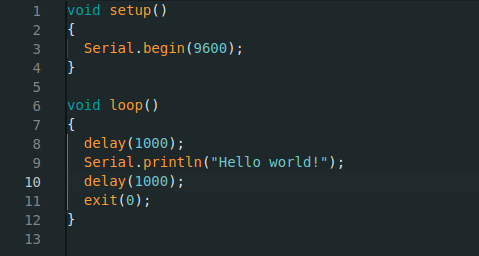
\includegraphics[width=0.9\textwidth]{pictures/code.png}
    	\caption{Ukázka kódu kdy Arduino posílá zprávu do IDE}
   	\label{fig:usbIDE}
\end{figure}

Na obrázku \ref{fig:usbIDE} je kód, který demonstruje jak se dá poslat text do IDE. V setupu je potřeba nastavit modulační rychlost, kdy 9600 je maximum pro Arduino. V metodě \hl{loop()} je pak samotný výstup, kdy sekundové čekání je moc, ale měl by se text vypisovat opakovaně, tak bude potřeba, jinak ho nebudeme stíhat číst.

\begin{figure}[H]
	\centering
	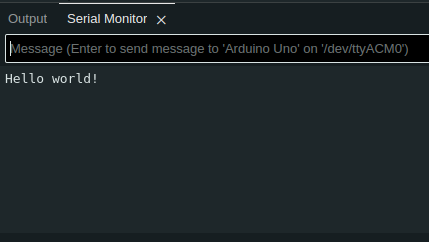
\includegraphics[width=0.9\textwidth]{pictures/message.png}
    	\caption{Ukázka výpisu zprávy z arduina}
   	\label{fig:msgIDE}
\end{figure}
Na obrázku \ref{fig:msgIDE} vidíme konzoli, která je ve spodní části IDE a je v ní text “Hello world!” z ukázky na obrázku \ref{fig:usbIDE}.


	
	
	\chapter{Použitý HW a SW}
	%!TeX root =  ../../thesis.tex

\section{Arduino}
Základem testeru je mikrokontrolér od značky Arduino model \ardMeg. Tento model disponuje velkým počtem pinům, na které je možné připojit různá zařízení a následně je ovládat mikrokontrolérem. Mikrokontroléry Arduino se programují pomocí C/C++. Já firmware pro toto tester píši v C++.

\begin{figure}[h!]
	\centering
	
\includegraphics[width=\textwidth]{pictures/placeHolderFHD.png}
    	\caption{\ardMeg}
   	\label{fig:arduinoMega}
\end{figure}


%\subsection*{Ino file}
%\lstinputlisting[language=C++, caption={Code.ino}, label={lst:code}]{../code/Code.ino}

%\subsubsection*{Co je to Ino file?}
%Ino file je soubor skatche pro Arduino, Arduino IDE ho využívá jako hlavní soubor, jen má místo metody main() metody setup() a loop().  Metoda setup() slouží pro přípravu zařízení a je automaticky volána při spuštění zaříze,  loop() pak obsahuje kód, který je vykonáván %mikrokontrolérem, dokud není vypnut nebo se nevyskytne problém. Arduino se dá programovat i pomocí svého upraveného jazyka C++, proto koncovka .ino.




	\newpage
	%!TeX root =  ../../thesis.tex

\section{Display}

Pro potřeby testeru byl vybrán standardní LCD displej se žlutým podsvícením o čtyřech řádcích po dvaceti znacích. Tento displej bude postačovat, jelikož je potřeba zobrazit menu, aby uživatel mohl vybrat typ kabelu dle koncových konektorů a následně výsledek testu, kterému jsou věnovány poslední dva řádky, na které se taky budou vypisovat chybová hlášení. V prvním řádku je vypsána verze programu a na poslední pozici bliká znak “\#”, který se objeví a zmizí vždy na jednu sekundu, z důvodu kontroly, že zařízení “nezamrzlo” a je možné jej bez problému použít.

\begin{figure}[H]
	\centering
	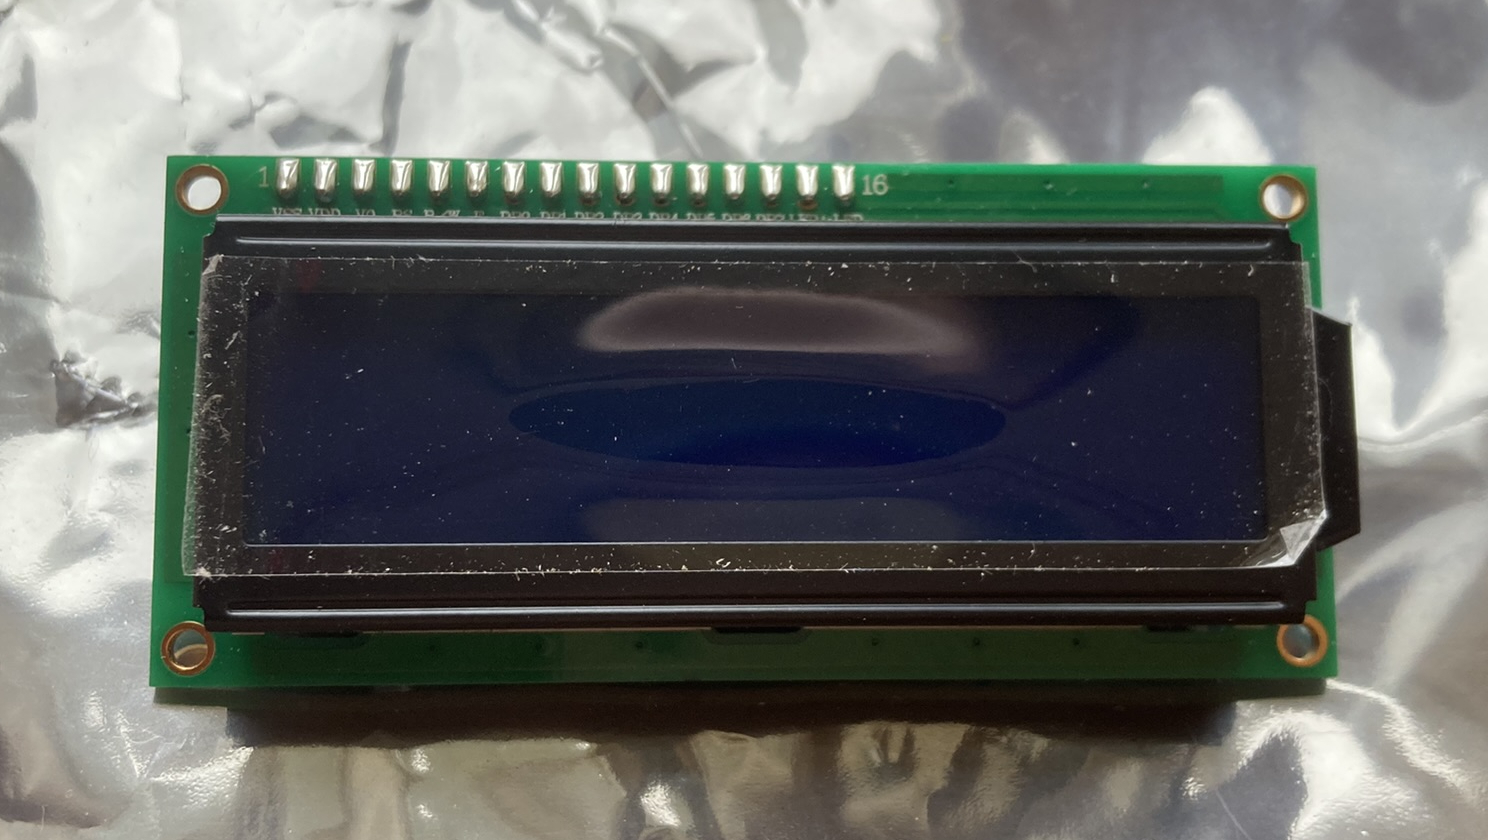
\includegraphics[width=0.9\textwidth]{pictures/display.jpeg}
    	\caption{Display}
   	\label{fig:displayHW}
\end{figure}

Na obrázku \ref{fig:displayHW} je displej, který sice není použitý pro tester, ale je to principiálně stejný displej a vlevo nahoře jsou vidět vrchní strany pinů, kterými se displej připojuje k Arduino nebo po případě k breadbordu.
	\newpage
	%!TeX root =  ../../thesis.tex

\section{Klávesnice}
\begin{figure}[h!]
	\centering
	
\includegraphics[width=\textwidth]{pictures/placeHolderFHD.png}
    	\caption{Klávesnička}
   	\label{fig:keyborad}
\end{figure}

\subsection{Připojení k desce}
\begin{table} [h!]
	\centering
	\catcode`\-=12 % Because of czech
	\begin{tabular}[c]{|| c | c | c ||}
	\hline
		\multicolumn{3}{||c||}{Piny klávesničky} \\
	\hline
 		 \textbf{PIN} & \textbf{Tlačítko} & \textbf{Akce}\\
	\hline
		42 &  RIGHT & Posune menu doprava\\
	\hline
		46 & POWER & N/A\\
	\hline
		48 & LEFT & Posune menu doleva\\
	\hline
		50 & MENU & N/A\\
	\hline
		52 & AUTO & Začne testovat vybraný kabel\\
	\hline
	\end{tabular}
	\caption{Pinové rozložení klávesnice}
	\label{table:pinKB}
\end{table}

\newpage
\subsection{Keyboard controller}
\lstinputlisting[language=C++, caption={Display controller}, label={lst:cpp_display}]{../code/src/components/Keyboard.h}

	
	\chapter{Návrh testeru kabelů – Hardwarová část}
	%!TeX root =  ../../thesis.tex

\section{Tester}
Tester je umístěn v plastovém boxu na vrchní části je umístěn displej a klávesnice na ovládání a na přední části jsou konektory pro testovaní kabelů.\\

Na obrázku \ref{fig:tester}  je pohled na výsledné testovací zařízení z vrchu, kdy je vidět celé ovládací rozhraní.
\\
Obrázek \ref{fig:testerIO} ukazuje konektory, kdy první tři zleva jsou výstupní a zbylé jsou vstupní, neboli ty testované.

\begin{figure}[H]
	\centering
	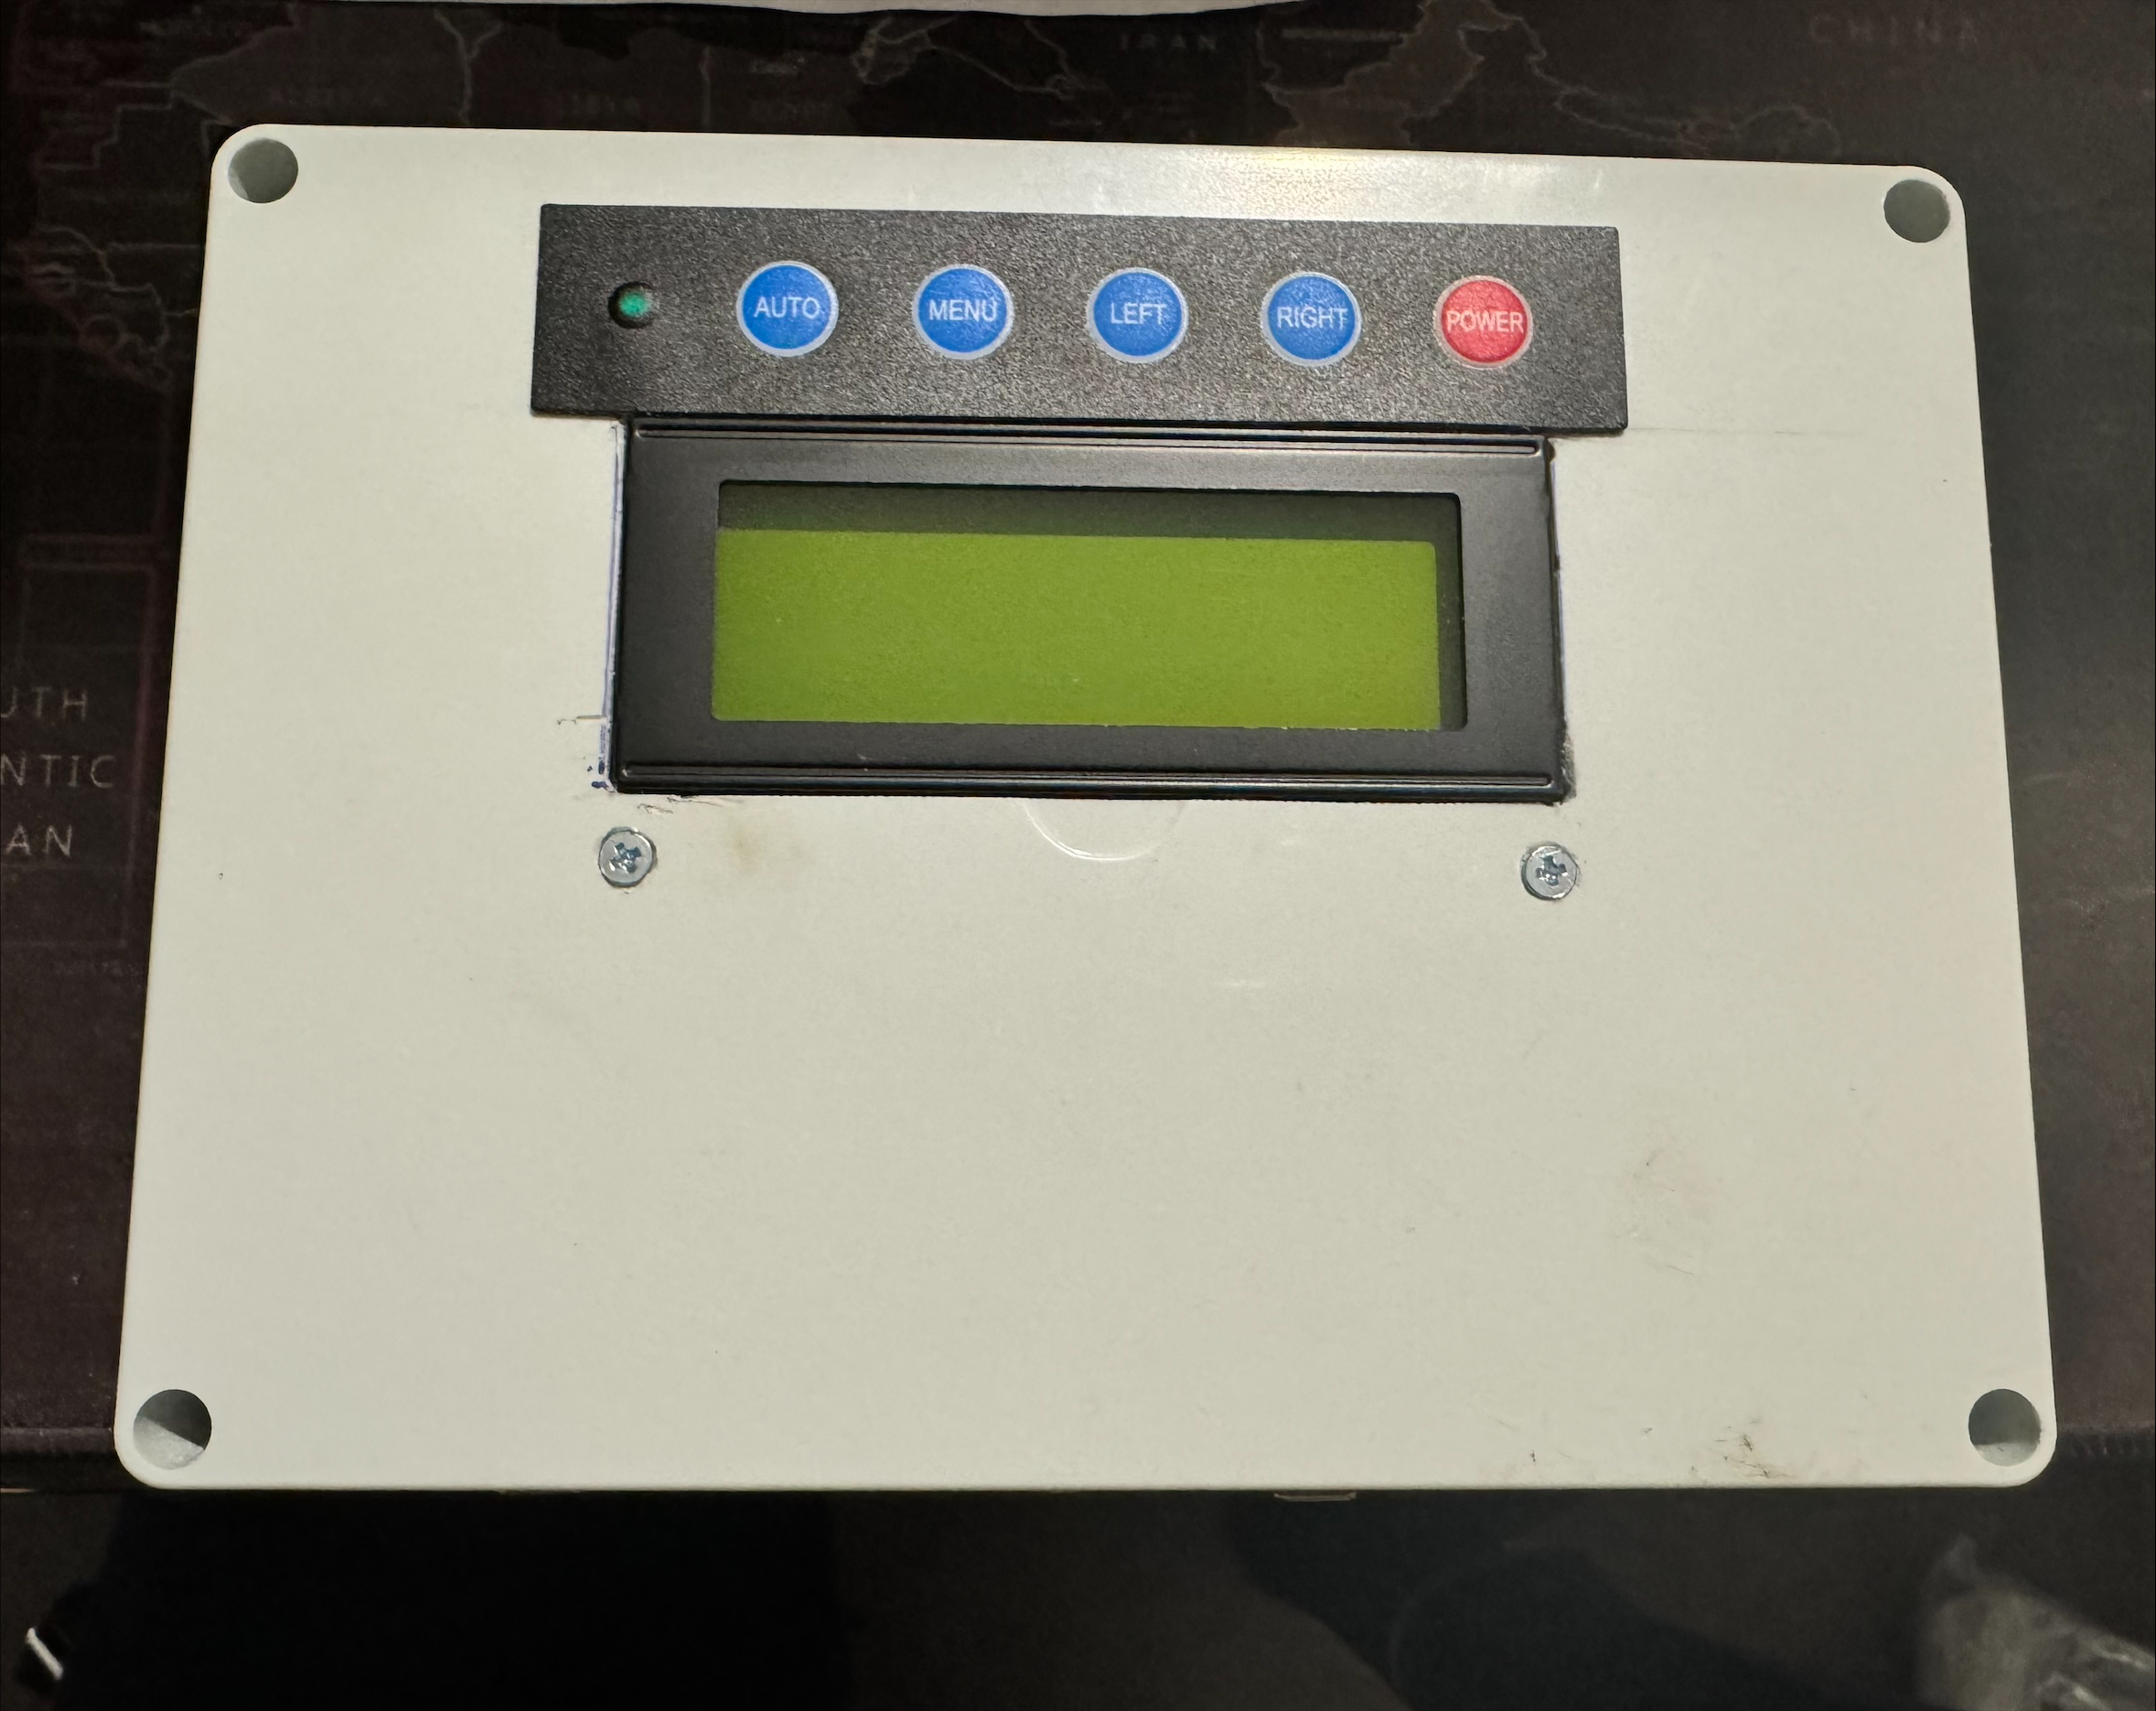
\includegraphics[width=0.9\textwidth]{pictures/tester-top.jpeg}
    	\caption{Výsledný tester na kabely}
   	\label{fig:tester}
\end{figure}

\begin{figure}[H]
	\centering
	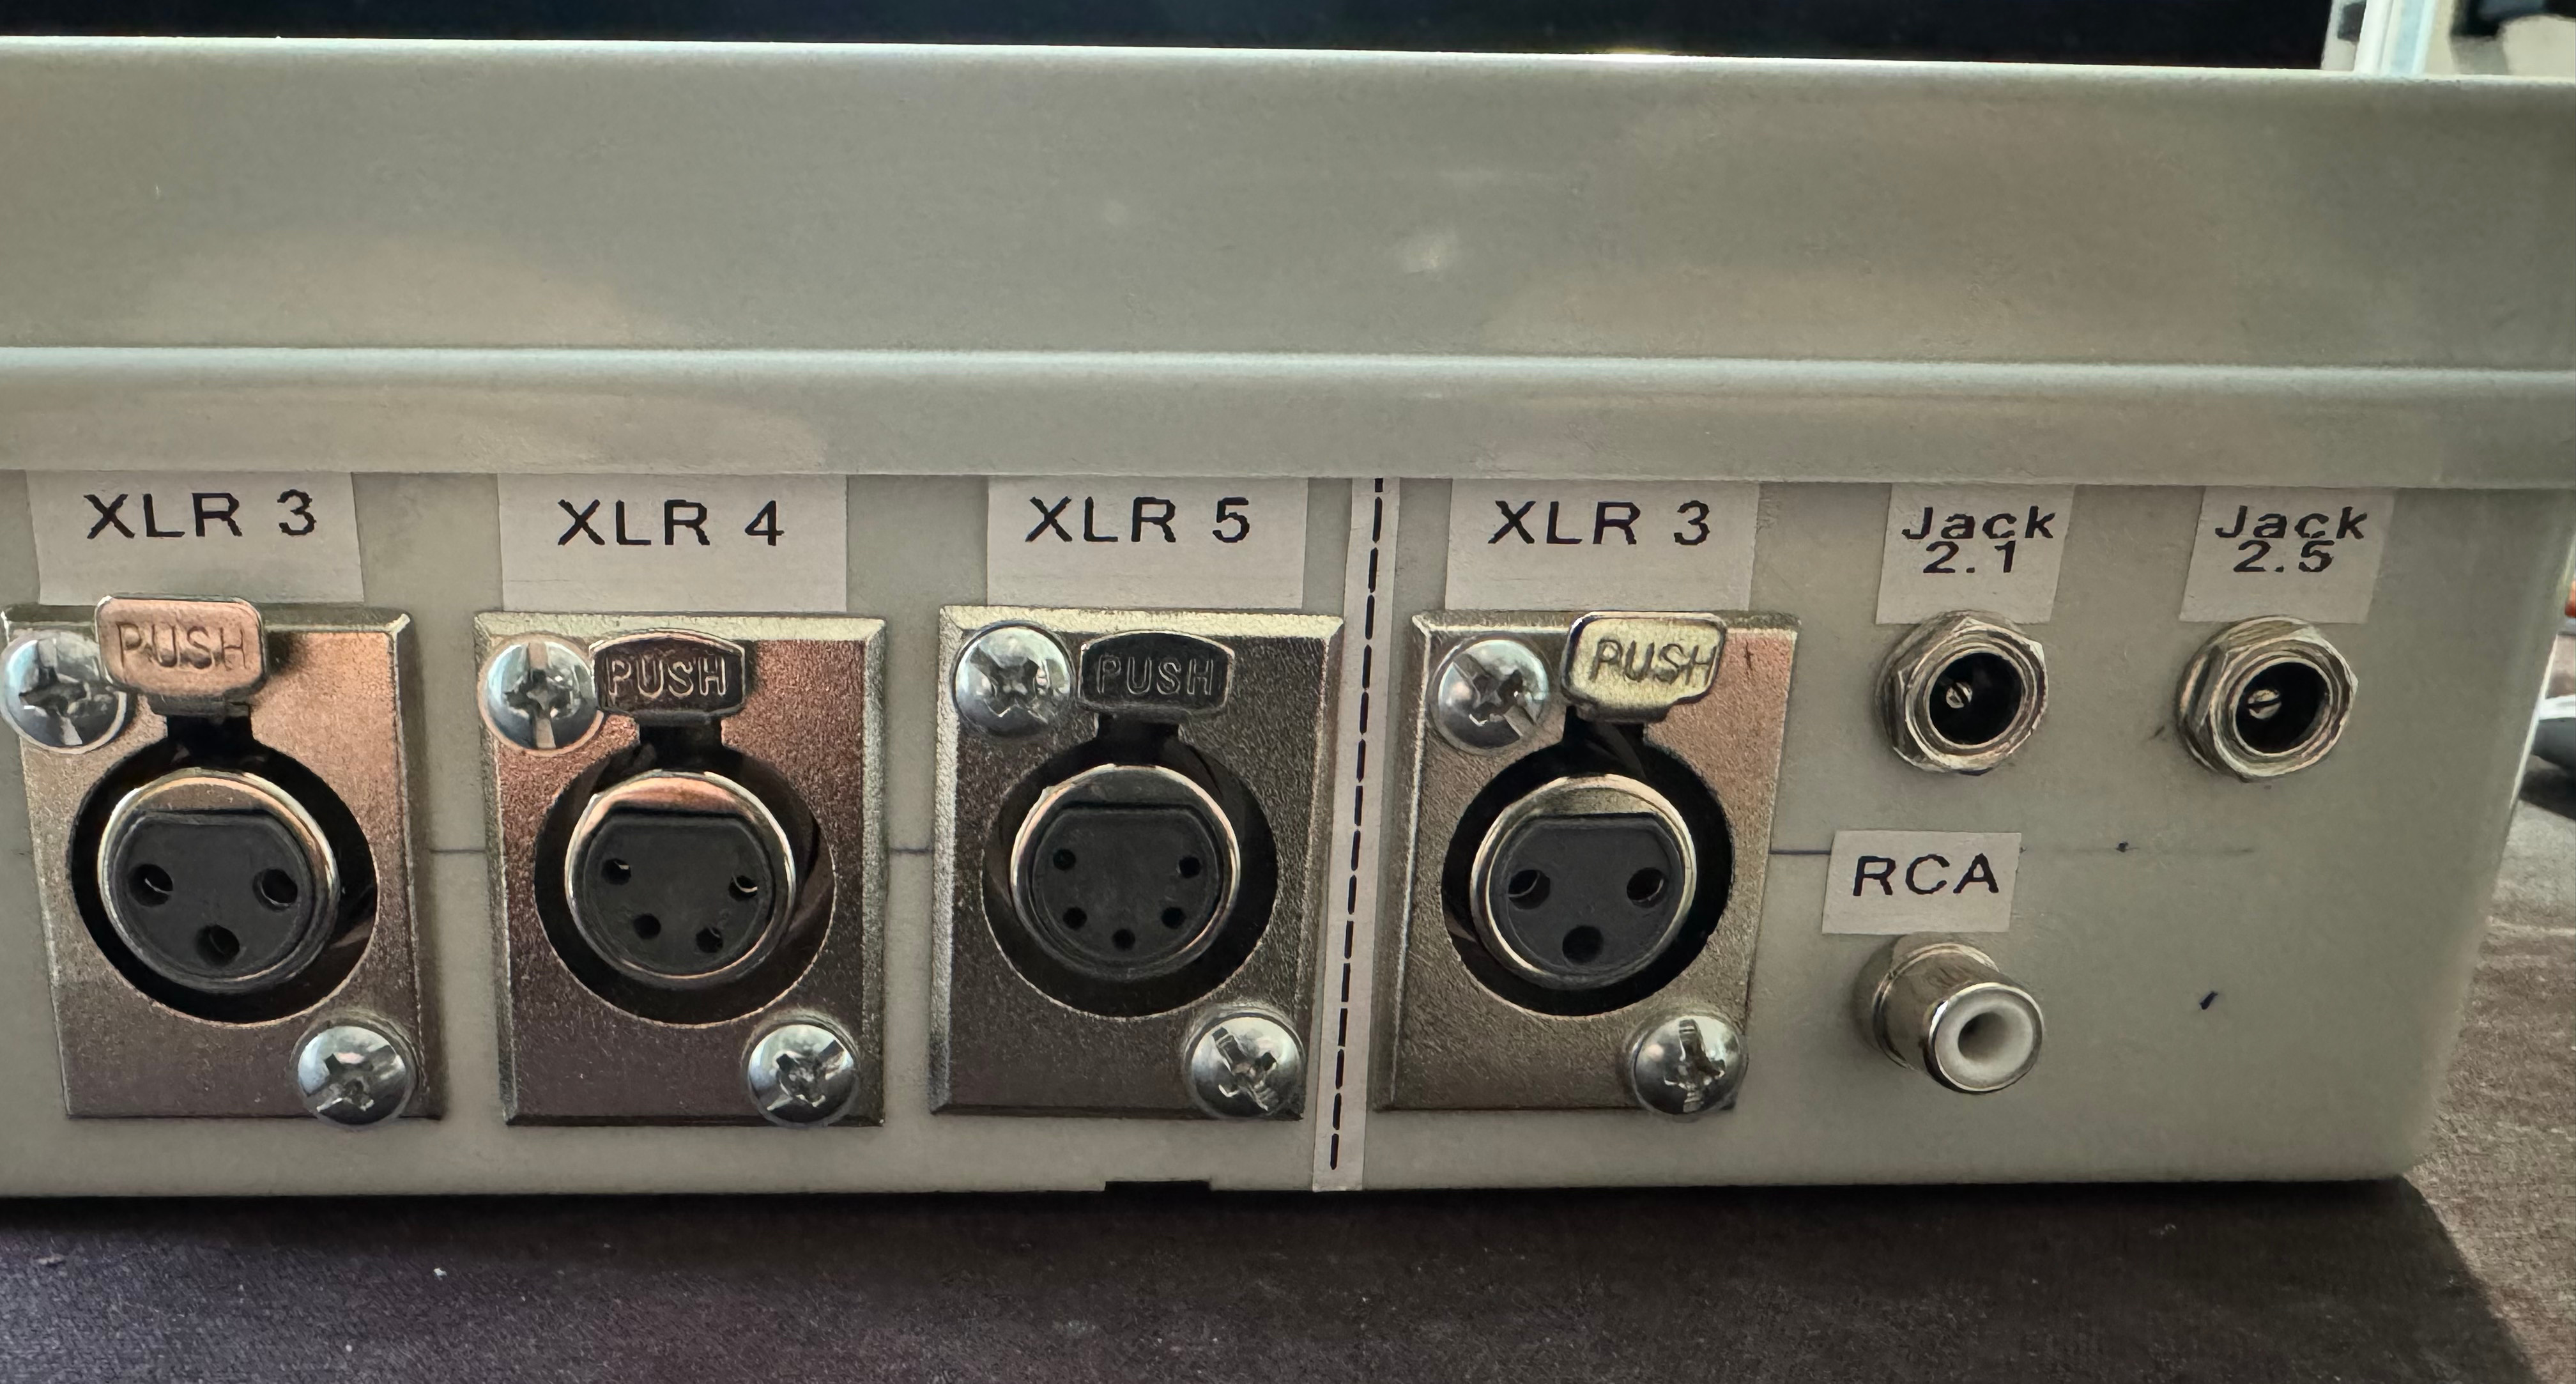
\includegraphics[width=0.9\textwidth]{pictures/tester-io.jpeg}
    	\caption{Výsledný tester na kabely}
   	\label{fig:testerIO}
\end{figure}


	
	\chapter{Návrh testeru kabelů – Softwarová část}
	%!TeX root =  ../../thesis.tex

\section{UML}

\section{Klíčové třídy}
\subsection{Controller}
Controller je hlavní třída, ačkoliv je hlavní část je v code.ino \ref{lst:code}, třída Controller zpřehlední kód, jelikož se do ní nic nedoplňuje při kompilaci, jako do hlavního ino souboru.

\subsection{Connector}
Společný předek pro konkrétní konektory.

\subsection{IComponent}
Společný předek pro komponenty zařízení, jako jsou například: displej, klávesnice nebo bzučák.

	
	
	\chapter{Testování}
	%!TeX root =  ../../thesis.tex

\section{Princip}
Principem testování je metoda “bool Connector::testConnector(char[])”, tato metoda posílá signál z pinu nastaveného na OUT a čte na pinu druhého konektoru, který je nastavený na “INPUT\_PULLUP”, což aktivuje interní rezistory, což eliminuje chybné čtení způsobeného elektrickým šumem od ostatních pinů. Pokud se podaří přečíst signál, tak je navýšena kontrolní hodnota, která musí být rovna počtu pinů na konektoru pro úspěšný test, tester tento test opakuje třikrát, aby se měření zpřesnilo. V případě, že se nepodaří přečíst signál na protilehlém pinu, tak je číslo pinu uloženo do pole na příslušnou pozici, navýšenou o jedna, aby se nepřepsala hodnota s návratovým kódem výsledku testu.
	
	
	\chapter{Závěr}
	Cílem práce bylo vytvořit zařízení pro testování nabíjecích kabelů pro elektrická kola s použitím mikrokontroléru Arduino. Výsledné zařízení je splňuje požadavky a je možné jednoduše rozšířit funkčnost díky objektovém přístupu v jazyce C++. Zařízení je schopné vypsat na displej přesně, které piny konektoru jsou špatné a nepřenáší se skrz ně elektrický proud/signál, také vypisuje chybové hlášky i v případě chybné implementace, například při nenastavení příslušných pinů pro konektor na Arduinu. Také pomocí zvuku upozorňuje zařízení uživatele na na výsledek testu a svého stavu, jsou naimplementované/ošetřené čtyři chybové stavy. Také na bezpečnost byl kladen důraz a přes kabel nejde více než 5V, které stačí, pro vyhodnocení testu.

	\newpage
	\chapter{Přílohy}
	\section*{Zdroje}
	\addcontentsline{toc}{section}{Seznam zdrojů}
	https://www.arduino.cc/en/about
	
	%\lstlistoflistings
	%\addcontentsline{toc}{section}{Seznam zdrojových kódů} % Add the list of listings to the TOC as a section

\end{document}